\documentclass[a4paper]{article}

\usepackage[english]{babel}
\usepackage[utf8x]{inputenc}
\usepackage[T1]{fontenc}

\usepackage[a4paper,top=3cm,bottom=2cm,left=3cm,right=3cm,marginparwidth=1.75cm]{geometry}

\usepackage{amsmath}
\usepackage{graphicx}
\usepackage[colorinlistoftodos]{todonotes}
\usepackage[colorlinks=true, allcolors=blue]{hyperref}
\usepackage{capt-of}
\usepackage{floatrow}
\floatsetup{heightadjust=object}
\newfloatcommand{capbtabbox}{table}[][\FBwidth]

\newcommand{\note}[1]{\marginpar{#1}}

%\setlength{\parindent}{0pt}

\title{Decision Trees\\\large{Mathematical Aspects of Machine Learning}}
\author{Florian Hartmann, Yu He}
\date{July 17, 2017}

\begin{document}
\maketitle

\section{Introduction}

Decision trees are a popular method in supervised Machine Learning. For this project phase, we decided to explore them in more detail and to apply them to some interesting datasets. Primarily, our motivation behind this was that decision trees are very interpretable. Part of the project is analyzing datasets, and we concluded that choosing an interpretable method would be quite helpful for doing that.

Before diving into the dataset analysis, this section introduces the foundational ideas behind decision trees. After having understood how to use decision trees, the more important question of how to build them is discussed in the next section, by looking at two popular algorithms. Section 3 deals with a popular heuristic for choosing the features that are used to make decisions.
The sections afterwards explain the technical details behind our decision tree visualization, and how ensemble methods can be used to combat overfitting. Finally, two datasets are analyzed using decision trees.

\todo{Create our own example image} A simple decision tree can be found in Figure \ref{fig:simple}. Decision trees consist of two types of nodes: First of all, internal nodes (i.e.\ nodes that are not leafs) make decisions based on features. Depending on the outcome of the decision, a different child node is visited next. At the bottom of the tree, there are leafs: They make very simple predictions, e.g.\ by just constantly predicting the same answer or by using a linear classifier. In the visualization, internal nodes are displayed using ellipses and leafs using rectangles. To make a prediction, a path down the decision tree is traversed until a leaf is reached. The leaf node is then asked to make the final prediction.

\begin{figure}
	\centering
	\includegraphics[scale=0.4]{dt.png}
    \caption{A simple decision tree}
    \label{fig:simple}
\end{figure}

Another way to think about this is that decision trees repeatedly split the input space, until the individual partitions allow for simple predictions. In computer science, this is known as a divide and conquer strategy. By making several subsequent decisions based on each other, nonlinear decision boundaries can easily be created.

There are many other useful traits of decision trees. For example, users have to perform very little data preprocessing. Feature values do not need to be normalized at all, and some decision tree algorithms can even deal with missing values by themselves.

As mentioned earlier, decision trees allow for easy interpretation. In contrast to other Machine Learning methods like neural networks, it is very clear why a prediction was made. For many applications, for example in the medical world, this interpretability is very important and a great advantage of decision trees.

By now it should be obvious that decision trees describe their training data very clearly. However, this also leads to the great disadvantage that decision trees overfit easily. In many cases, they learn to describe the training data exactly, and their predictions do not generalize well to unseen data. Several sections of this report deal with methods that aim to reduce this problem.

Finally, it is worth noting that we focus on classification in this report. Nevertheless, decision trees can also be used for regression, e.g.\ by using linear regression models in the leaf.

\section{Constructing Decision Trees}

\subsection{ID3}

ID3 (Iterative Dichotomiser 3) is a straight-forward approach for building decision trees. We decided to start with this algorithm because it allows for a gentle introduction to the fundamental ideas behind building decision trees.
The fact that it is quite simple also means that it has some serious drawbacks, and generally should not be used in production. We will explain these shortcomings and address the most important ones in later sections of the report.

Generally, ID3 implements the ideas introduced in the previous section. There are two types of nodes: Internal nodes that make the decision which node to visit next, and leafs  which make a constant prediction.
To build a decision tree using ID3, a recursive strategy is followed: The training data is repeatedly split until a new node gets training data that is suitable for making a constant prediction.

In the following, we will look at both of these type of nodes, starting with internal nodes.

\subsubsection{Internal nodes: Making decisions}

In ID3, the input data is always split based on a single feature. For each possible value of that feature a new child node is created.
In other words, if a split is made on a feature that allows $k$ different values, then the node will have exactly $k$ child nodes.
The child nodes then build their own subtrees using the subset of the training data from the parent node that has the respective value in the selected feature.

Here the first serious drawback of ID3 becomes apparent: Splitting on all possible values only works well for categorical features. For a continuous variable like \emph{age} this approach would work terribly. This is also the major shortcoming of ID3. In Section \ref{subsec:c45}, we will see an algorithm that deals with continuous features in a smarter way.

\subsubsection{Leafs: Stopping the recursion}

At some point, the recursion has to end, which means a node does not grow a subtree but is turned into a leaf. The leaf then constantly predicts the same answer. Which answer to predict is based on the training data it received.

There are various reasons why a node might be turned into a leaf. The simplest one is that all data points it received have the same label. In this case, there is no reason to split the data further, and the node can be turned into a leaf which predicts this label. A comparable case is that the training data does not allow for any further splits, e.g.\ if all data points are equal to each other but have different labels. In this case, the most common label is predicted.

Another case is that there is just no training data available. We always create a new node for each possible value of a feature. If we are deep in the tree and split on a feature that can have many different values, there might be no training data for some values. If this happens, the most common label of the parent node is predicted.

There are other cases where we might want to stop the recursion. We will come back to these in Section \ref{subsec:id3-depth}.

\subsubsection{Selecting the feature to split on}

Of course, now the major remaining question is how find the best feature to split on. ID3 follows a greedy strategy for this. For each feature, it evaluates how well the classes would be divided in the next step if a split based on this feature would be performed. Then, the feature where this worked best is chosen. Of course, this greedy strategy could mean that a very good combination of subsequent splits is missed, because we were too greedy in the beginning.

To find the feature which produces the best division in the next step, different heuristics can be used. The easiest one is misclassification: We just assume that the next node will predict the most common label and calculate how accurate it would be by doing this. Then, the feature with the lowest misclassification rate is chosen.

A more popular heuristic that is also used in ID3 is entropy with information gain. In a nutshell, entropy measures uncertainty, i.e.\ it wants nodes to receive data points that mostly have the same label so that a prediction can be made with a lot of certainty. Because entropy and information gain are not only used in ID3, but also in C4.5, a more thorough description of it is given in Section~\ref{sec:entropy}.

Another important idea to mention is that in ID3 each feature should only be used once for splitting. Because we split based on all possible values, the data of each child only has one kind of value for each feature that was already split on. Hence, it does not make sense to split on these features again.

\subsubsection{Limiting the tree depth}
\label{subsec:id3-depth}

Overfitting is a huge problem with decision trees. It can happen very easily that the training data is perfectly described. However, this description might contain so much noise that the predictions don not generalize well for previously unseen data points.

In most Machine Learning algorithms a very common way to combat overfitting is regularization: By adding additional constraints, the model is forced to be simpler. A simpler model means there is less capacity for remembering information from the training data, and hopefully the more important information is remembered.

For decision trees, the primary way to add regularization is to limit the tree depth. Because we split on each feature exactly once, limiting the tree depth in ID3 is equivalent to limiting the maximum number of features that should be used for one prediction. If only a low tree depth is allowed, it means that only the most important features are considered. Instead of splitting, a leaf is then created that predicts the most common label.

Of course, the optimal tree depth highly depends on the dataset being used. Because of this, tree depth is a hyperparameter that needs be optimized by a method like cross validation.

Another way to limit the tree depth is to only perform a split if the information gain is high enough. The intuition behind this is that splits with low information gain tend to introduce more model complexity without directly improving the predictive power of the model.

However, sometimes a split with low information gain is necessary to get a good split afterwards. One extreme example for this is the xor dataset, see Table \ref{fig:xor-table}. We have two features, $a$ and $b$ that take the values of $0$ and $1$. The label is computed using the $\mathit{xor}$ function. Ideally, our decision tree should look like the one in Figure \ref{fig:xor-tree}.

However, in the first layer of the tree, all possible ID3 splits yield an information gain of $0$, as they do not improve the division of classes at all. If we stop here, we could only get an accuracy of 50\%, which is equivalent to randomly guessing. However, if we perform the split without a direct information gain, we can perform a perfect split afterwards, which yields an information gain of 1 and improves the accuracy to 100\%.

\begin{figure}
\begin{floatrow}
\ffigbox{%
  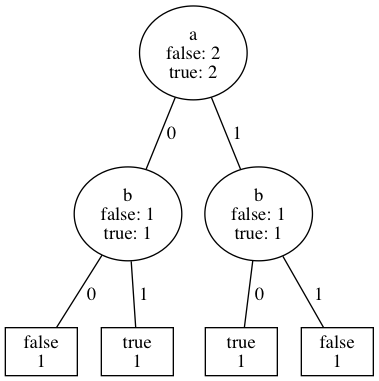
\includegraphics[scale=0.4]{xor.png}%
}{%
\caption{xor decision tree}%
	\label{fig:xor-tree}
}
\capbtabbox{%
  \begin{tabular}{c|c|c}
      \textbf{a} & \textbf{b} &  \textbf{y = a xor b} \\
      \hline
      0 & 0 & false \\
      0 & 1 & true  \\
      1 & 0 & true \\
      1 & 1 & false
  \end{tabular}
}{%
\caption{xor truth table}%
	\label{fig:xor-table}
}
\end{floatrow}
\end{figure}

\subsection{C4.5}
\label{subsec:c45}

C4.5 is a more advanced decision tree algorithm that was designed to fix many of ID3's shortcomings. It was created by Ross Quinlan, who also invented ID3. Quinlan wrote an entire book on C4.5, so to reimplement all ideas and variations of C4.5 is beyond the scope of this project. Instead, we will focus on the three ideas that we consider to be the most central ones.

\subsubsection{Continuous features}

As we saw in the previous section, ID3 can only deal well with discrete features. However, most datasets contain continuous features. Always throwing these features away or manually converting them into discrete features is of course not an optimal solution. C4.5 fixes this shortcoming, which is probably the greatest improvement of C4.5 to ID3.

Before we start explaining how the splitting works, it is worth taking a moment to think about how the algorithm actually knows whether a feature is discrete or continuous. Because we are only working on some samples, it is impossible to always automatically detect this correctly. One could imagine checking how many different values a feature has, and then just considering it as continuous if it has more than a certain number of different values. However, this process is very error-prone. Zip codes would probably be considered continuous, although they come from a discrete set. In the end, we just decided that the user should tell the algorithm which features should be treated as continuous features.

If a feature is continuous, we of course do not want to split on all possible values. Instead, C4.5 always considers a binary split by comparing the feature value to a split constant $h$. In other words, the data is partitioned using $\le h$ and $> h$.

It is straight-forward to come up with a bruteforce solution for finding a suitable $h$: We just consider all values in the training set that this feature can take, and then calculate the information gain we get by each of these splits. Then, the maximum information gain for this feature is compared to the ones from other features.

While this can lead to a good value of $h$, it is also easy to see that this is a bad solution if the training set is large enough. It turns out that it is also not necessary as many values for $h$ will lead to the same splits for the training data, so they can be considered equivalent. For an example of this, see Figure \ref{fig:continuous-feature}. The bruteforce solution here would be to check the information gain for $h = 0, \dots, 5$. However, $h = 0$ and $h = 1$ lead to the exact same partitoning of the data, similarly $h = 2, \dots, 4$ are equivalent to each other, and only one of these values has to be tried. There are different ways to choose this one value, the most common one is to calculate the mean. So for this dataset, one would try the splits given by $h = 0.5, 3, 5$.

To deal with this, we wrote a helper function that generates all splits that are useful to consider. Neighbouring values that only have the same single class are grouped together for one split. Values that have more than one label (e.g. $5$ in our example) are always considered for a split.

\begin{figure}
	\centering
  \begin{tabular}{l|l}
      \textbf{Feature value} & \textbf{Label} \\
      \hline
      0 & A \\
      1 & A \\
      2 & B \\
      3 & B \\
      4 & B \\
      5 & A \\
      5 & B
  \end{tabular}

  \caption{Example data for a continuous feature}
  \label{fig:continuous-feature}
\end{figure}

\subsubsection{Missing values}

Most algorithms in Machine Learning do not know how to deal with missing features by themselves. So usually, the user has to deal with the misssing values before giving the data to the algorithm, e.g. by always imputing the mean value for the respective feature.

C4.5 has a built-in way to deal with this problem, so that the user does not have to deal with it at all. First of all, missing values are ignored when computing information gain. When splitting on a feature, it is also remembered how common the individual options for the split are. This gives us a probability distribution, where we can choose a child node randomly, weighted by how commonly that child node is accessed.

When wanting to make a decision based on a missing feature, we just use this probability distribution to choose the next child node to visit. This has an effect similiar to imputing the most common (or the mean) value of that feature, except it is not done on a global level anymore. Instead, the imputing is just based on the training data the respective node was given, and now there is also some randomness involved.

While training, the data points with a missing value can be divided in the same random way. An alternative is to give data with missing values preferedly to child nodes that have very few data points using the normal splitting. By doing this, the individual child nodes all have enough data to make good predictions. Of course, this can also wrongly introduced biases, so one needs to be careful. In the end, one should use cross validation to see which settings works better.

Sometimes, it is important to always predict the same answer. The deterministic variant of this algorithm, is to always choose the most common option when predicting, except of sampling the probability distribution.

\subsubsection{Pruning}

As explained earlier, deep decision trees are incredibly prone to overfitting. For this reason, trees are commonly stopped from growing if they get too deep. However, because of the greedy approach we do not really know which nodes to grow further beforehand. As we saw in the xor example, growing the tree as far as possible is often required to see if a split actually yielded a good result because it enabled a good split a few steps later.

This is the central idea behind pruning: In the first step, we grow the tree as far as possible. Afterwards, we traverse the tree again and turn internal nodes into leafs when they do not improve the predictive accuracy of the model.

There are many variants of how this can be done. We decided to implement one based on cross validation. After fitting the model using training data, the user can call a special method for pruning that accepts a validation set. This validation set is then used to test what nodes actually improve the accuracy.

An inverse breadth-first search is performed, so we first go through the nodes at the bottom of the tree. We then turn each node individually into a leaf, and compare the accuracy of the model before with the new one, both times using the validation set. If the change improved the accuracy, the node is kept as a leaf, otherwise it is turned back into an internal node. This process is done for the entire tree.

Intuitively, this makes a lot of sense. The complexity of the model is reduced unless that complexity actually helps to improve the accuracy of unseen data.

\section{Entropy and Information Gain}
\label{sec:entropy}

To find the feature which leads to the best split in the current iteration, both ID3 and C4.5 use entropy and information gain. Entropy takes a list of values and computes how much uncertainty there is in this information. In other words, if the list only contains the same values, then there is no uncertainty on what to predict and the entropy would be $0$. If the list only contains two different values at the same frequency, then the prediction without any further information can not be better than a coin throw, so the entropy is $0.5$. In a formula, entropy is calculated like this:\todo{If we have enough space, a 2d plot of entropy would be nice here}
\[
	H(S) = \sum\limits_{i = 1}^J p_i * \log_2\left(\frac{1}{p_i}\right)
\]

\noindent where we loop over all $J$ different values the labels that the dataset $S$ contains, and $p_i$ is the probability of the $i$-th label occuring.

Now, let's assume we split on a feature $a$. In ID3 and C4.5, we split on all possible values for $a$, which we call the set $V(a)$ in the following. For each split the recursive process is then followed. To compute how good this split is, we assume that in the next level of the subtree, only constant predictions will be made. How well, the constant predictions can be made can be computed using entropy.

We need to aggregate the information of how well the split works over all different children the split on $a$ would produce. This is called information gain, and it is a measure for how good a split is, a larger value implying more gain from a split:
\[
	\mathit{IG}(S, a) = H(S) - \sum\limits_{v \in V(a)} P_{a, v} * H(S_v)
\]

\noindent where $S$ is the entire dataset and $P_{a, v}$ is the probability that feature $a$ has value $v$.

The intuition behind this is that a split is good if it reduces the uncertainty. So we compare the current uncertainty with the one a split on this feature would yield. The individual entropy calculations are weighted by how common they are.

\section{Drawing Decision Trees}

\todo{Add about a third of a page here, max one half}

\section{Random Forest}

As already noted in other sections, decision trees are very prone to overfitting. One idea to combat this is to regularize the depth. This makes decision trees weak learners, i.e.\ they have little capacity for learning much information and make simple decisions. A popular ensemble method in Machine Learning is bagging, for combining many weak learners into a strong learner.

One example for this is a majority classifier: It takes a bunch of already trained models, ideally these are all weak learners. For prediction, it then lets each classifier vote on the answer and then predicts the answer with a relative majority. The individual classifiers have a bad accuracy, but by making them vote we can still recognize the most important pattern. Overfitting is harder here, because if many classifiers agree on a prediction, there is probably enough evidence for it in the data.

Random Forest is a way of applying this idea to decision trees: A set of decision trees (i.e.\ a forest) is trained, each on different subsets of the data, and then they are given to a majority classifier. In theory, this does not have to be much slower than training normal decision trees, because this process can be parallelized well. We did not do this here, so it did increase training time quite a bit.

There are two popular ways to choose what data to train the individual trees on: One is to train them on different data points, the other to train them on different features. We implemented both of these methods. These subsets of data or features are chosen randomly, hence the name Random Forest.

Generally, training them on different features seems to be the most popular method in literature, and it also worked better for us. However, this introduces a large amount of randomness. By training the same forest several times, we now got quite different results. Some forests had too many trees that got bad features, so they performed very badly.

Because of this, we had the additional idea to let the user specify a prior weighting to features. By doing this, we can ensure that interesting features are used for more trees. If the user has no prior knowledge, a uniform distribution is used. Of course ideally we would want to infer feature importance automatically, but this is also a lot more complicated. In our case, it also was not necessary as we had good ideas what features for our two example datasets might be promising.

One problem with random forest is that there are now a lot more hyperparameters to optimize for: The number of trees to use, how the training data is selected, if we want to weight features, if pruning should be used or the depth should be limited. In order to optimize for all of these, a lot more training time is required. Random forest also makes our models a bit harder to interpret.

\section{Evaluating datasets}

\subsection{Titanic}

\begin{itemize}
	\item Give a short introduction to the dataset
    \item Use ID3 and C4.5, show visualization with max depth 2, and report accuracy, compare with sklearn
    \item C4.5: Compare imputing with just using missing values (improves test accuracy, makes training accuracy worse)
    \item C4.5: Report how pruning and max depth help, maybe in form of a table with different accuracies
    \item Report how well random forest does, compare with sklearn
    \item Test how accuracy changes when different features get removed and then report what feature are most important
\end{itemize}

\subsection{Income census}

\begin{itemize}
	\item describe a little bit about the dataset

    The dataset is from UCI machine learning repository. Extraction was done by Barry Becker from 1994 Census database. The attribute information includes age, workclass, education and so on. The prediction task is to predict whether a person can make over 50K a year.


	\item show the result of using income census dataset with ID3 and C4.5

	First we used ID3 and C4.5 to construct decision trees with different maximum depth. The accuracy of each tree are shown below.

	It is clear that with the growing depth of decision tree constructed by ID3, the accuracy drops from 0.8227 to 0.8184. On the contrary, the accuracy of decision trees built by C4.5 grows when their depths grow.

    The reason why this situation happened could be

	\item remove one feature from the feature list, for example using either education or occupation, then show the result and explain the result.

    Another experiment we did is to use a subset of features for training our decision tree. We consider that the feature "relationship" is redundant to another feature "marital-status", so we removed one of them, and tested the model after we trained it. The decision trees in this experiment are all with maximum depth of 3. The accuracy of both trees are shown below.

    The last experiment is directly removing the feature "native country", because this feature in dataset includes 41  kinds of values. With such many detailed values the model can cause overfitting. After we removed it, the accuracy of the decision tree built by ID3 dropt to 0.7637, but the accuracy of the decision tree built by C4.5 grows to 0.8345. The reason why the accuracy dorps in ID3 tree can probably be that the number of discrete features is only 8, including feature "native-country". When we removed feature "native-country", there are only 7 left. Such few features cause underfitting. This situation will not happen in C4.5 model, because in C4.5 model there are 12 discrete or continuous features. Even if we remove the feature "native-country", there are still 11 features left, which underfitting will not happen. Meanwhile, overfitting is also avoided by that removal of that feature. That is why the accuracy grows to be the highest in C4.5 model.

\end{itemize}

\bibliographystyle{alpha}
\bibliography{sample}
\todo{We still need to collect the sources we used}

\end{document}
